\section{模型拟合}
\subsection{数据源}
\par 拟合所用数据为2020年1月20日至5月1日官方发布的全国疫情数据。
以下为官方发布的疫情数据:
\begin{figure}[H]
    \centering
    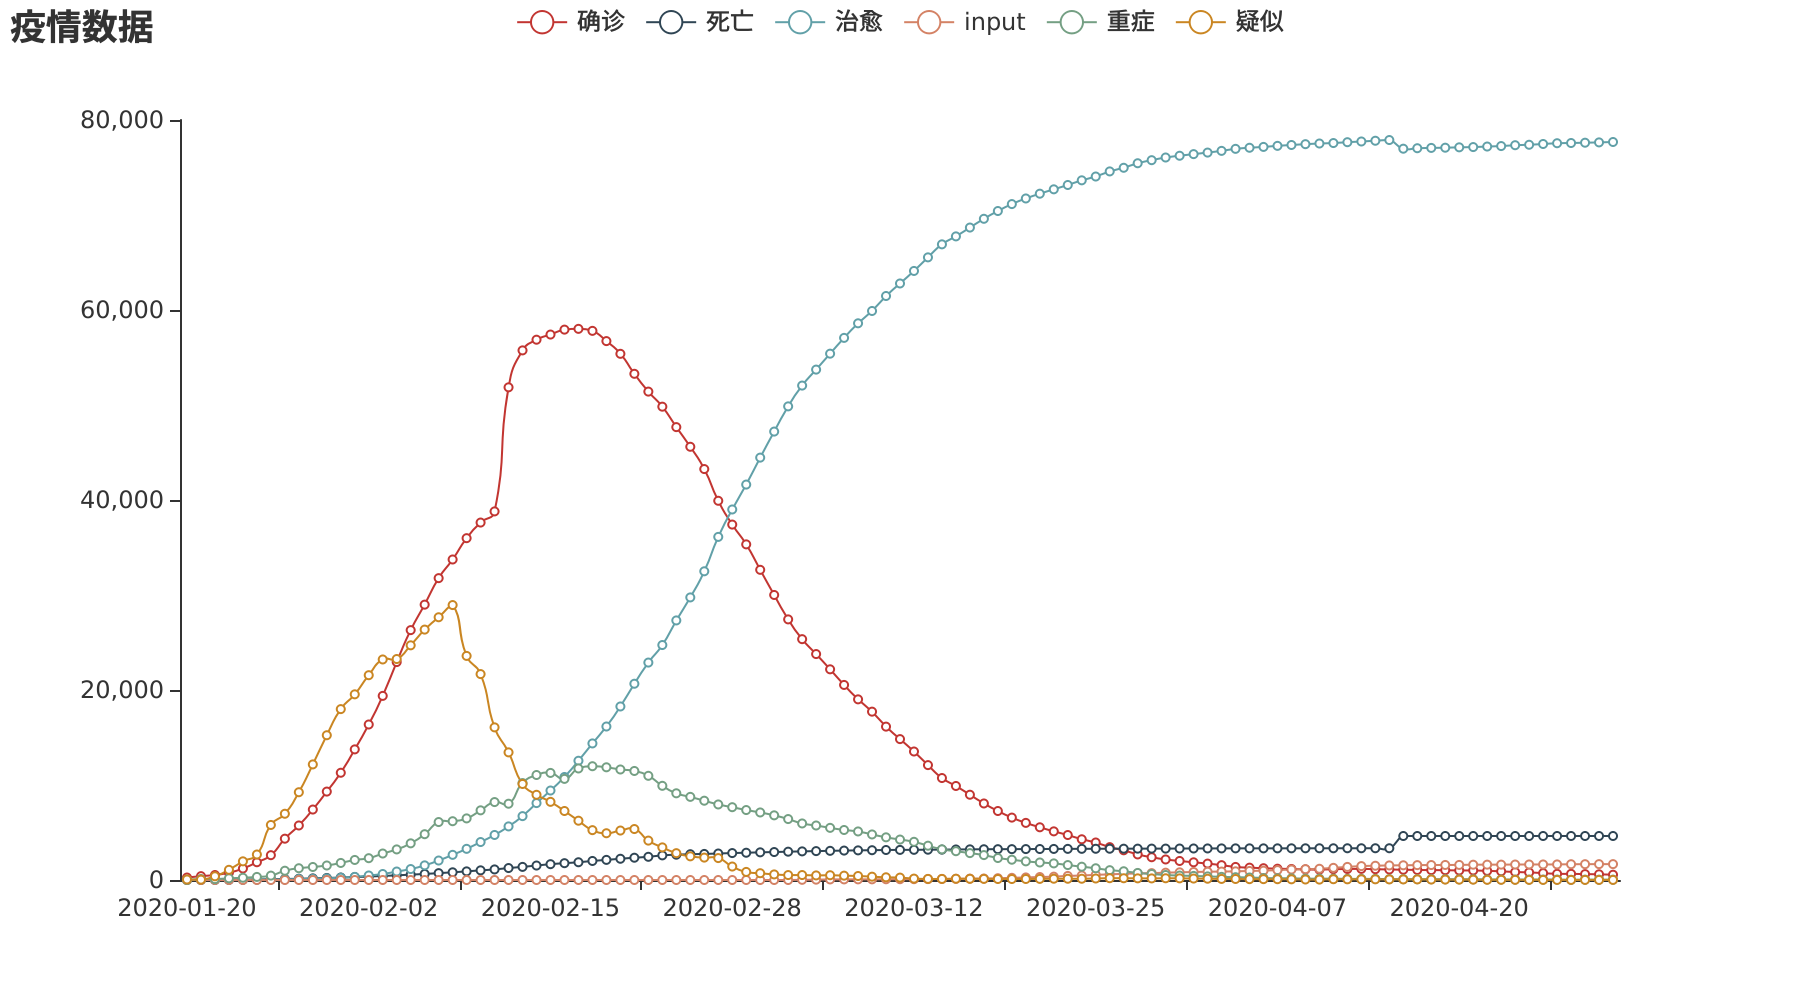
\includegraphics[width=\imagewidth]{疫情数据.png}
    \caption{全国疫情数据\label{figure:全国疫情数据}}
\end{figure}
\begin{figure}[H]
    \centering
    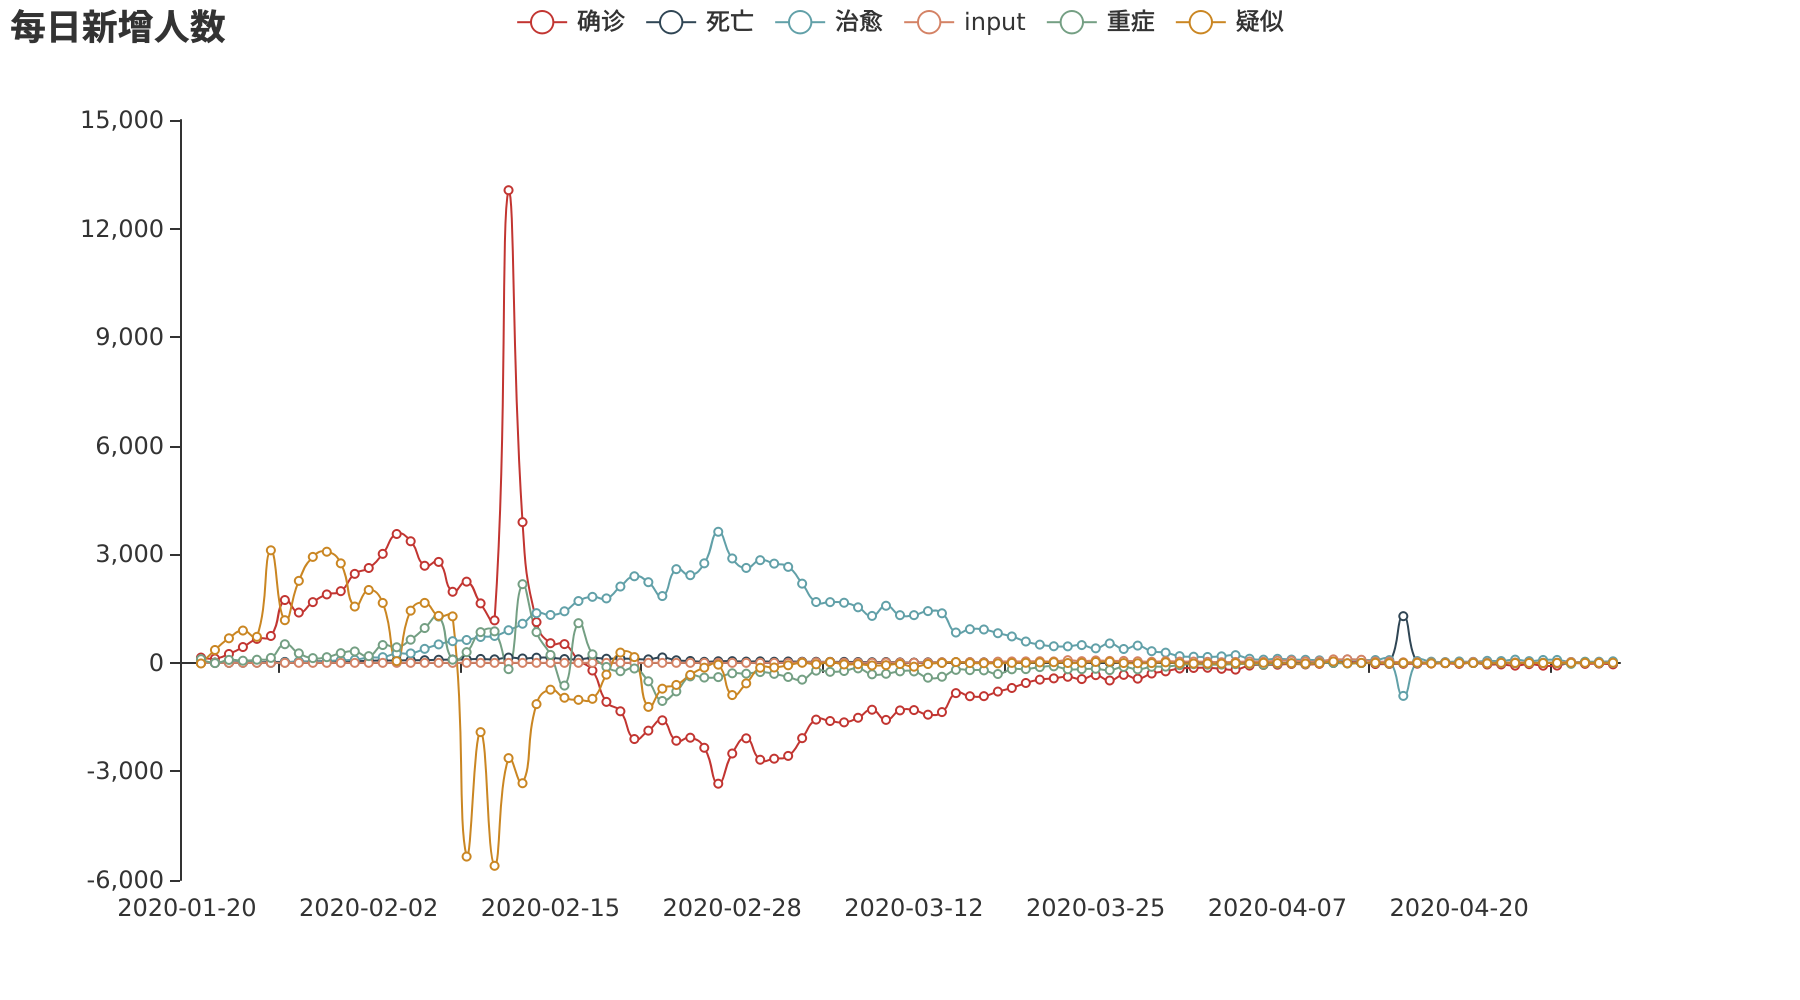
\includegraphics[width=\imagewidth]{每日新增人数.png}
    \caption{每日新增人数\label{figure:每日新增人数}}
\end{figure}
\par
由图\ref{figure:全国疫情数据}及图\ref{figure:每日新增人数}可见,
2月12日确诊人数猛增,
是因为当日重新规定了确诊条件,
导致许多疑似病例纳入确诊人数。
\subsection{拟合方法}
\par 本文采取$L-BFGS-B$方法对每个模型进行拟合,
将每个模型的模拟值与真实数据进行对比,
并给出拟合后的参数以及损失值$LOSS$和拟合度$FIT$,
损失值代表了模型拟合的优劣程度,
拟合度代表了模型预测的忧劣程度,
损失值和拟合度将作为本文评判模型优劣的指标。
\par 本文采用2020年1月20日至2020年5月日的数据进行拟合,
采用前$70\%$的数据进行训练并计算$LOSS$值,
后$30\%$的数据进行验证并计算$FIT$值。
\par 损失值及拟合度定义:
\begin{equation}
    LOSS= FIT = \frac{\sum\limits^{day}\sum\limits^{group}
        (True-Predict)^2}{day}
    \label{math:LOSS}
\end{equation}
\par 式(\ref{math:LOSS})中,
$True$为真实数据,
$Predict$为预测数据,
$LOSS$和$FIT$为计算预测值与真实值的方差后取均值的结果。
\subsection{SIR模型拟合结果}
\showtable{SIR}
\par 因拟合数据较长,将其放在附录\ref{append:数据表},
故在此以图像的形式展示模型拟合结果。
带有“预测”字样的为拟合数据曲线,
不带“预测”字样的为真实数据曲线,
例如在图\ref{figure:SIR模型拟合图像}中,
“预测确诊”和“预测治愈”为模型拟合数据,
“确诊”和“治愈”为真实数据。
\showfigure{SIR}
\par $SIR$模型(表\ref{table:SIR模型拟合参数}、图\ref{figure:SIR模型拟合图像})中$\P{S}{I}$为感染人数增长率,
不同于感染率。
$\P{I}{R}$为治愈人数增长率,
不同于治愈率。
\subsection{SEIR模型拟合结果}
\showtable{SEIR}
\showfigure{SEIR}
\par $SEIR$模型(表\ref{table:SEIR模型拟合参数}、图\ref{figure:SEIR模型拟合图像})中$\P{E}{R}$极低,
一可理解为潜伏期较长,
二可理解为致病率较高,
这两点都与实际情况吻合。
\subsection{SEIRD模型拟合结果}
\showtable{SEIRD}
\showfigure{SEIRD}
\par $SEIRD$模型(表\ref{table:SEIRD模型拟合参数}、图\ref{figure:SEIRD模型拟合图像})中$\P{I}{D}$为预测死亡增长率,
不同于死亡率。
\subsection{SEIRS模型拟合结果}
\showtable{SEIRS}
\showfigure{SEIRS}
\par $SEIRS$模型(表\ref{table:SEIRS模型拟合参数}、图\ref{figure:SEIRS模型拟合图像})中的$\P{R}{I}=0.001$,
可以理解为复阳率极低,
说明复阳人数占患病人数比例极低,
对疫情的影响微乎其微。
\subsection{考虑隔离的模型拟合结果}
\par 对比各个模型拟合前后的参数值变化:
\showtables{SIR}
\showfigures{SIR}
\par 在$SIR$模型(表\ref{table:SIR模型隔离前后拟合参数}、图\ref{figure:SIR模型隔离前后拟合图像})中,
$\P{S}{I}$有所下降,
$\P{I}{R}$有所增减,
代表感染率降低,
治愈率提高。
\showtables{SEIR}
\showfigures{SEIR}
\par 在$SEIR$模型(表\ref{table:SEIR模型隔离前后拟合参数}、图\ref{figure:SEIR模型隔离前后拟合图像})中,
$\P{S}{E},\P{E}{I}$有所下降,
$\P{I}{R}$有所增减,
代表感染率降低,
治愈率提高。
\showtables{SEIRD}
\showfigures{SEIRD}
\par 在$SEIRD$模型(表\ref{table:SEIRD模型隔离前后拟合参数}、图\ref{figure:SEIRD模型隔离前后拟合图像})中,
$\P{S}{E}$、
$\P{E}{I}$有所下降,
$\P{S}{E}\cdot \P{E}{I}$有所下降,
$\P{I}{R}$有所增加,
$\P{I}{D}$有所下降
代表患病率降低,
治愈率提高,
死亡率降低。
\showtables{SEIRS}
\showfigures{SEIRS}
\par $SEIRS$模型(表\ref{table:SEIRS模型隔离前后拟合参数}、图\ref{figure:SEIRS模型隔离前后拟合图像})
与$SEIRD$模型(表\ref{table:SEIRD模型隔离前后拟合参数}、图\ref{figure:SEIRD模型隔离前后拟合图像})
的参数十分接近,
无论分段与否,$SEIRS$模型的$\P{S}{I}$均为$0.001$,
说明$\P{S}{I}$对模型的影响极其微弱。
\subsection{结果分析}
\par 仅从$LOSS$值判断,
模型从优到劣排序为$SEIRD>SEIRS>SEIR>SIR$。
\par 仅从$FIT$值判断,
模型从优到劣排序为$SEIRD>SIR>SEIR>SEIRS$。
\par 综合考虑$LOSS$值及$FIT$值的大小,
认为在上述几种模型中,
$SEIRD$模型最适用于该类传染病预测。
\par 无论哪种模型,
比较模型分段前后参数,
均可得出传染病的传染率降低、治愈率增加、死亡率降低这一结论。
\par 本文使用基础再生数$R_0$和有效再生数$R_t$两个参数来评估疫情传播情况:
\par 基础再生数$R_0$为自然状态下,
平均一个患者可以传染的人数。
$R_0$常用来描述疫情传播速率,
可以通过$R_0$来反映一个传染病的爆发力和严重程度。
\par 有效再生数$R_t$是指加上防控手段后,
平均一个患者可以传染的人数,
$R_t$的计算公式与$R_0$相同。
\par $R_0$($R_t$)的计算公式为\cite{应用SEIR模型预测2009年甲型H1N1流感流行趋势,王宝童2013流感传播数学模型的基本再生数}:
\begin{equation}
    R_0(R_t) = \frac{\P{S}{I}}{\P{I}{R}}
    = \frac{\P{S}{E}\cdot \P{E}{I}}{\P{I}{R}}
    \label{math:R0计算公式}
\end{equation}
\par 根据表\ref{table:SEIRD模型拟合参数}依据式(\ref{math:R0计算公式})
可计算出总体的有效生殖数$R_t=\ro$
与官方发布数据$1.4\sim 3.8$相符。
\par 根据表\ref{table:SEIRD模型隔离前后拟合参数}计算出隔离前基本生殖数$R_0=\ro$及隔离后有效生殖数$R_t=\rt$,
可见在防控措施下疫情传播得到了有效遏制。
其中计算所得$R_0$符合疫情早期爆发情况下的基本生殖数估计值$4.16\leq R_0\leq 7.10$\cite{协调基本生殖数量及其不确定性的早期暴发估计:新型冠状病毒(SARS-CoV-2)暴发的框架和应用},
略高于2020年2月8日前的基本生殖数估计值$3.63\leq R_0\leq 5.13$\cite{估计2019年新型冠状病毒的流行性:数学建模研究},
考虑到本文以2020年2月12日为分界线,
此时正处于疫情爆发时间,
所得结论可以接受。
